% !TEX root=./adl.tex

% ---------------------------------------------------------------------------
%  Shared TikZ styles and colours for attention illustrations
% ---------------------------------------------------------------------------
\tikzset{
  acell/.style={minimum width=0.26cm, minimum height=0.26cm,
                draw=gray!50, inner sep=0, line width=0.3pt},
  attn arrow/.style={-{Stealth[length=3pt,width=2.5pt]}, gray!60, thin},
}
\colorlet{xcol}{green!40}
\colorlet{qcol}{violet!30}
\colorlet{kcol}{orange!35}
\colorlet{vcol}{cyan!25}
\colorlet{zcol}{pink!50}

\section{Attention \& Transformers}

\subsection{Self-Attention}

% -----------------------------------------------------------------------
\begin{frame}{Motivation: Why Attention?}
  Consider the sentence:
  \begin{center}
    \textit{``The animal didn't cross the street because \textbf{it} was too tired.''}
  \end{center}

  To understand what \textbf{it} refers to, a model must connect it to \textbf{animal}, five tokens away.

  \vspace{0.5em}
  \textbf{The challenge:} When processing a sequence, each token must be able to selectively gather
  information from \emph{any} other token, regardless of distance.

  \begin{itemize}
    \item RNNs pass information through a fixed-size hidden state, a bottleneck for long-range dependencies.
    \item \textbf{Attention} provides a direct, learnable connection between any two positions.
    \item Each token asks: \emph{``Which other tokens are relevant to me, and how much?''}
    \item The answer is computed dynamically from the content of the tokens themselves.
  \end{itemize}

  \vspace{0.3em}
  \begin{block}{References}
    \begin{itemize}
      \item \cite{vaswani2017attention}
      \item \cite{alammar2018illustrated}
    \end{itemize}
  \end{block}
\end{frame}

% -----------------------------------------------------------------------
\begin{frame}{Token Embeddings}
  \begin{itemize}
    \item Each token is mapped to a learnable feature vector, its \textbf{token embedding}.
    \item The embedding matrix $E \in \mathbb{R}^{V \times d}$ is a lookup table: row $i$ gives the embedding for token $i$.
  \end{itemize}

  \begin{center}
  \begin{tikzpicture}[scale=0.95,
      tok/.style={draw=gray!50, rounded corners=2pt, minimum width=1.1cm,
                  minimum height=0.45cm, font=\small, fill=white, inner sep=3pt},
      arr/.style={-{Stealth[length=3pt]}, gray!60, thin},
    ]

    % ---- Layout ----
    % Two tokens: "Thinking" and "Machines"
    % Embedding vector: 4 cells of 0.36 cm = 1.44 cm wide
    % Vector centre offset from token centre: 4*0.36/2 = 0.72, first cell at -0.72+0.18
    % Token 1 centre x = 1.5,  Token 2 centre x = 4.5
    \def\tA{1.5}   % centre x of token 1
    \def\tB{4.5}   % centre x of token 2
    \def\vecw{0.36} % cell width/height
    \def\nd{4}      % number of embedding dims shown

    % ---- Token labels ----
    \node[tok, font=\small\bfseries, text=green!60!black] (tokA) at (\tA, 3.15) {Thinking};
    \node[tok, font=\small\bfseries, text=green!60!black] (tokB) at (\tB, 3.15) {Machines};

    % ---- Embedding matrix E on the left ----
    \node[font=\small\bfseries, text=green!60!black] at (-2.05, 3.55) {$E$};
    \foreach \ri in {0,...,6} {
      \foreach \ci in {0,...,3} {
        \pgfmathsetmacro{\cy}{2.90 - \ri*0.26 + 0.13}
        \pgfmathsetmacro{\cx}{-1.70 + \ci*0.26 + 0.13}
        \pgfmathtruncatemacro{\isHL}{(\ri == 2 || \ri == 5) ? 1 : 0}
        \ifnum\isHL=1
          \node[acell, fill=xcol, draw=green!50!black] at (\cx, \cy) {};
        \else
          \node[acell, fill=gray!12] at (\cx, \cy) {};
        \fi
      }
    }
    \node[font=\small, gray] at (-1.30, 1.01) {\vdots};
    \node[font=\tiny, text=green!60!black, anchor=west] (idx1) at (-0.48, 2.90-2*0.26+0.13) {$i_1$};
    \node[font=\tiny, text=green!60!black, anchor=west] (idx2) at (-0.48, 2.90-5*0.26+0.13) {$i_2$};
    % Connect token IDs to their token labels
    \draw[dashed, green!50!black, thin, -{Stealth[length=2.5pt]}]
      (idx1.east) to[out=0, in=200] (tokA.south west);
    \draw[dashed, green!50!black, thin, -{Stealth[length=2.5pt]}]
      (idx2.east) to[out=0, in=210] (tokB.south west);
    % Top brace for d (columns)
    \draw[decorate, decoration={brace, amplitude=3pt}, gray, thin]
      (-1.70, 3.20) -- (-0.66, 3.20)
      node[midway, above=3pt, font=\scriptsize, gray] {$d$};
    % Left brace for V (rows)
    \draw[decorate, decoration={brace, amplitude=3pt, mirror}, gray, thin]
      (-1.78, 3.16) -- (-1.78, 1.34)
      node[midway, left=5pt, font=\scriptsize, gray] {$V$};

    % ---- Embedding vectors (centred below each token label) ----
    % Token 1
    \node[font=\small, text=green!60!black, anchor=east]
      at (\tA - \nd*\vecw/2 - 0.08, 2.0) {$x_1$};
    \foreach \ci in {0,...,3} {
      \pgfmathsetmacro{\cx}{\tA - \nd*\vecw/2 + \ci*\vecw + \vecw/2}
      \node[acell, minimum width=\vecw cm, minimum height=\vecw cm,
            fill=xcol, draw=green!50!black] at (\cx, 2.0) {};
    }
    \draw[arr] (\tA, 2.92) -- (\tA, 2.20);

    % Token 2
    \node[font=\small, text=green!60!black, anchor=east]
      at (\tB - \nd*\vecw/2 - 0.08, 2.0) {$x_2$};
    \foreach \ci in {0,...,3} {
      \pgfmathsetmacro{\cx}{\tB - \nd*\vecw/2 + \ci*\vecw + \vecw/2}
      \node[acell, minimum width=\vecw cm, minimum height=\vecw cm,
            fill=xcol, draw=green!50!black] at (\cx, 2.0) {};
    }
    \draw[arr] (\tB, 2.92) -- (\tB, 2.20);

    % ---- Dimension brace (under token 1's vector) ----
    \pgfmathsetmacro{\brL}{\tA - \nd*\vecw/2}
    \pgfmathsetmacro{\brR}{\tA + \nd*\vecw/2}
    \draw[decorate, decoration={brace, amplitude=4pt, mirror}, gray!60, thin]
      (\brL, 1.78) -- (\brR, 1.78)
      node[midway, below=5pt, font=\scriptsize, gray] {$d$ dimensions};

    % ---- Vocab annotation ----
    \node[font=\scriptsize, gray, align=center] at (-1.30, 0.60)
      {$V$ tokens\\in vocab};

  \end{tikzpicture}
  \end{center}
\end{frame}

% -----------------------------------------------------------------------
\begin{frame}{Self-Attention: Queries, Keys, and Values}
  Each token $i$ projects its embedding $x_i \in \mathbb{R}^d$ into three vectors via learned matrices:

  \begin{columns}[T]
    \begin{column}{0.40\textwidth}
      \vspace{0.5em}
      \begin{itemize}\itemsep0.6em
        \item \textbf{\textcolor{violet!80!black}{Query}} $q_i = x_i W^Q$\\[2pt]
              {\small ``What am I looking for?''}
        \item \textbf{\textcolor{orange!80!black}{Key}} $k_i = x_i W^K$\\[2pt]
              {\small ``What do I contain?''}
        \item \textbf{\textcolor{cyan!60!black}{Value}} $v_i = x_i W^V$\\[2pt]
              {\small ``What will I contribute?''}
      \end{itemize}
      \vspace{0.6em}
      {\small $W^Q, W^K, W^V \!\in\! \mathbb{R}^{d \times d_k}$ are shared across all tokens.}
    \end{column}
    \begin{column}{0.58\textwidth}
      \begin{center}
      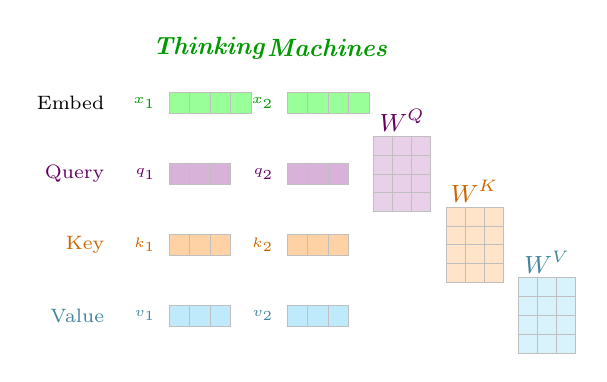
\begin{tikzpicture}
        % cell = 0.26 cm square
        % embed (d=4):  4 cells = 1.04 cm wide
        % qkv   (dk=3): 3 cells = 0.78 cm wide
        % tok1 left-x = 0.55,  tok2 left-x = 2.05
        % W-boxes at x-center = 3.60
        % row y-centers: title=4.10, embed=3.40, q=2.50, k=1.60, v=0.70

        % ---- token name labels ----
        \node[font=\small\bfseries, text=green!60!black] at (0.55+0.52, 4.10) {\textit{Thinking}};
        \node[font=\small\bfseries, text=green!60!black] at (2.05+0.52, 4.10) {\textit{Machines}};

        % ---- row labels (far left, clear of subscript labels) ----
        \node[font=\scriptsize, anchor=east]                       at (-0.15, 3.40) {Embed};
        \node[font=\scriptsize, anchor=east, text=violet!80!black] at (-0.15, 2.50) {Query};
        \node[font=\scriptsize, anchor=east, text=orange!80!black] at (-0.15, 1.60) {Key};
        \node[font=\scriptsize, anchor=east, text=cyan!60!black]   at (-0.15, 0.70) {Value};

        % ---- TOKEN 1 ----
        \node[font=\tiny, text=green!60!black,   anchor=east] at (0.50, 3.40) {$x_1$};
        \foreach \ci in {0,...,3} {
          \pgfmathsetmacro{\cx}{0.55 + \ci*0.26 + 0.13}
          \node[acell, fill=xcol] at (\cx, 3.40) {};
        }
        \node[font=\tiny, text=violet!80!black,  anchor=east] at (0.50, 2.50) {$q_1$};
        \foreach \ci in {0,...,2} {
          \pgfmathsetmacro{\cx}{0.55 + \ci*0.26 + 0.13}
          \node[acell, fill=qcol] at (\cx, 2.50) {};
        }
        \node[font=\tiny, text=orange!80!black,  anchor=east] at (0.50, 1.60) {$k_1$};
        \foreach \ci in {0,...,2} {
          \pgfmathsetmacro{\cx}{0.55 + \ci*0.26 + 0.13}
          \node[acell, fill=kcol] at (\cx, 1.60) {};
        }
        \node[font=\tiny, text=cyan!60!black,    anchor=east] at (0.50, 0.70) {$v_1$};
        \foreach \ci in {0,...,2} {
          \pgfmathsetmacro{\cx}{0.55 + \ci*0.26 + 0.13}
          \node[acell, fill=vcol] at (\cx, 0.70) {};
        }

        % ---- TOKEN 2 ----
        \node[font=\tiny, text=green!60!black,   anchor=east] at (2.00, 3.40) {$x_2$};
        \foreach \ci in {0,...,3} {
          \pgfmathsetmacro{\cx}{2.05 + \ci*0.26 + 0.13}
          \node[acell, fill=xcol] at (\cx, 3.40) {};
        }
        \node[font=\tiny, text=violet!80!black,  anchor=east] at (2.00, 2.50) {$q_2$};
        \foreach \ci in {0,...,2} {
          \pgfmathsetmacro{\cx}{2.05 + \ci*0.26 + 0.13}
          \node[acell, fill=qcol] at (\cx, 2.50) {};
        }
        \node[font=\tiny, text=orange!80!black,  anchor=east] at (2.00, 1.60) {$k_2$};
        \foreach \ci in {0,...,2} {
          \pgfmathsetmacro{\cx}{2.05 + \ci*0.26 + 0.13}
          \node[acell, fill=kcol] at (\cx, 1.60) {};
        }
        \node[font=\tiny, text=cyan!60!black,    anchor=east] at (2.00, 0.70) {$v_2$};
        \foreach \ci in {0,...,2} {
          \pgfmathsetmacro{\cx}{2.05 + \ci*0.26 + 0.13}
          \node[acell, fill=vcol] at (\cx, 0.70) {};
        }

        % ---- WEIGHT MATRICES (gridded, staggered diagonally) ----
        % Each W is d×dk = 4 rows × 3 cols (0.24 cm cells).
        % They are offset horizontally so their y-ranges never overlap.
        % Each matrix is vertically centred at its own row (Q=2.50, K=1.60, V=0.70).
        %   matrix height = 4×0.24 = 0.96 cm  → half = 0.48 cm
        %   W^Q x-start = 3.15, bottom-y = 2.02
        %   W^K x-start = 4.07, bottom-y = 1.12
        %   W^V x-start = 4.99, bottom-y = 0.22

        % W^Q  (4 rows × 3 cols, centred at Q row y=2.50)
        \node[font=\small\bfseries, text=violet!80!black] at (3.51, 3.18) {$W^Q$};
        \foreach \ri in {0,...,3} {
          \foreach \ci in {0,...,2} {
            \pgfmathsetmacro{\cx}{3.15 + \ci*0.24 + 0.12}
            \pgfmathsetmacro{\cy}{2.02 + \ri*0.24 + 0.12}
            \node[acell, minimum width=0.24cm, minimum height=0.24cm,
                  fill=qcol!60] at (\cx, \cy) {};
          }
        }
        % W^K  (4 rows × 3 cols, centred at K row y=1.60)
        \node[font=\small\bfseries, text=orange!80!black] at (4.43, 2.28) {$W^K$};
        \foreach \ri in {0,...,3} {
          \foreach \ci in {0,...,2} {
            \pgfmathsetmacro{\cx}{4.07 + \ci*0.24 + 0.12}
            \pgfmathsetmacro{\cy}{1.12 + \ri*0.24 + 0.12}
            \node[acell, minimum width=0.24cm, minimum height=0.24cm,
                  fill=kcol!60] at (\cx, \cy) {};
          }
        }
        % W^V  (4 rows × 3 cols, centred at V row y=0.70)
        \node[font=\small\bfseries, text=cyan!60!black] at (5.35, 1.38) {$W^V$};
        \foreach \ri in {0,...,3} {
          \foreach \ci in {0,...,2} {
            \pgfmathsetmacro{\cx}{4.99 + \ci*0.24 + 0.12}
            \pgfmathsetmacro{\cy}{0.22 + \ri*0.24 + 0.12}
            \node[acell, minimum width=0.24cm, minimum height=0.24cm,
                  fill=vcol!60] at (\cx, \cy) {};
          }
        }
      \end{tikzpicture}
      \end{center}
    \end{column}
  \end{columns}
\end{frame}

% -----------------------------------------------------------------------
\begin{frame}{Self-Attention: Computing Scores}
  The \textbf{attention score} from token $i$ to token $j$ is the dot product of their query and key:
  \[
    s_{ij} = q_i^\top k_j
  \]

  \begin{columns}[T]
    \begin{column}{0.46\textwidth}
      \vspace{0.2em}
      \begin{center}
      \begin{tikzpicture}[scale=0.92]
        % Layout: 2 token columns, rows for query / key / value
        % Highlight box around token 2 ("Machines") — the active query
        % Arrows from q2 to k1 and k2

        % ---- token labels ----
        \node[font=\small\bfseries, text=green!60!black]  at (1.50, 3.50) {\textit{Thinking}};
        \node[font=\small\bfseries, text=violet!80!black] at (3.80, 3.50) {\textit{Machines}};

        % ---- row labels (far left, no overlap with subscripts) ----
        \node[font=\scriptsize, anchor=east, text=violet!80!black] at (0.35, 2.80) {Query};
        \node[font=\scriptsize, anchor=east, text=orange!80!black] at (0.35, 1.90) {Key};
        \node[font=\scriptsize, anchor=east, text=cyan!60!black]   at (0.35, 1.00) {Value};

        % ---- token 1 vectors ----
        \node[font=\tiny, text=violet!80!black, anchor=east] at (0.90, 2.80) {$q_1$};
        \foreach \ci in {0,...,2} {
          \pgfmathsetmacro{\cx}{0.95 + \ci*0.36 + 0.18}
          \node[acell, minimum width=0.36cm, minimum height=0.36cm,
                fill=qcol] at (\cx, 2.80) {};
        }
        \node[font=\tiny, text=orange!80!black, anchor=east] at (0.90, 1.90) {$k_1$};
        \foreach \ci in {0,...,2} {
          \pgfmathsetmacro{\cx}{0.95 + \ci*0.36 + 0.18}
          \node[acell, minimum width=0.36cm, minimum height=0.36cm,
                fill=kcol] at (\cx, 1.90) {};
        }
        \node[font=\tiny, text=cyan!60!black, anchor=east] at (0.90, 1.00) {$v_1$};
        \foreach \ci in {0,...,2} {
          \pgfmathsetmacro{\cx}{0.95 + \ci*0.36 + 0.18}
          \node[acell, minimum width=0.36cm, minimum height=0.36cm,
                fill=vcol] at (\cx, 1.00) {};
        }

        % ---- token 2 vectors ----
        \node[font=\tiny, text=violet!80!black, anchor=east] at (3.20, 2.80) {$q_2$};
        \foreach \ci in {0,...,2} {
          \pgfmathsetmacro{\cx}{3.25 + \ci*0.36 + 0.18}
          \node[acell, minimum width=0.36cm, minimum height=0.36cm,
                fill=qcol, draw=violet!60, line width=0.6pt] at (\cx, 2.80) {};
        }
        \node[font=\tiny, text=orange!80!black, anchor=east] at (3.20, 1.90) {$k_2$};
        \foreach \ci in {0,...,2} {
          \pgfmathsetmacro{\cx}{3.25 + \ci*0.36 + 0.18}
          \node[acell, minimum width=0.36cm, minimum height=0.36cm,
                fill=kcol] at (\cx, 1.90) {};
        }
        \node[font=\tiny, text=cyan!60!black, anchor=east] at (3.20, 1.00) {$v_2$};
        \foreach \ci in {0,...,2} {
          \pgfmathsetmacro{\cx}{3.25 + \ci*0.36 + 0.18}
          \node[acell, minimum width=0.36cm, minimum height=0.36cm,
                fill=vcol] at (\cx, 1.00) {};
        }

        % ---- highlight box centred on token-2 cells (the active query) ----
        \draw[violet!50, rounded corners=3pt, line width=1.2pt, dashed]
          (3.13, 0.60) rectangle (4.45, 3.20);

        % ---- score arrows from q2 (curved) ----
        % q2·k1 = 56 (high score)
        \draw[-{Stealth[length=5pt,width=4pt]}, violet!70, line width=0.8pt]
          (3.61, 2.60) to[out=-150, in=30] (1.49, 2.10);
        \node[font=\small\bfseries, text=violet!70!black] at (1.49, 0.35)
          {$q_2 \!\cdot\! k_1 = \mathbf{56}$};

        % q2·k2 = 38 (lower score)
        \draw[-{Stealth[length=5pt,width=4pt]}, violet!70, line width=0.8pt]
          (3.79, 2.60) to[out=-70, in=110] (3.79, 2.10);
        \node[font=\small, text=violet!50!black] at (3.80, 0.35)
          {$q_2 \!\cdot\! k_2 = 38$};

      \end{tikzpicture}
      \end{center}
    \end{column}
    \begin{column}{0.52\textwidth}
      \vspace{0.2em}
      {\small\textbf{Numerical example} ($d_k = 3$):}

      \begin{center}
      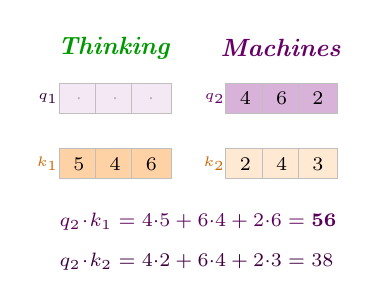
\begin{tikzpicture}[scale=0.92,
          val/.style={font=\scriptsize, minimum width=0.50cm, minimum height=0.38cm,
                      draw=gray!50, inner sep=0, line width=0.3pt}
        ]
        % Same layout as left: token columns, rows for q / k
        % q2 = [3, 7, 4],  k1 = [4, 6, 2] → 12+42+8=62 … adjust
        % q2 = [4, 6, 2],  k1 = [5, 4, 6] → 20+24+12=56 ✓
        % q2 = [4, 6, 2],  k2 = [3, 3, 5] → 12+18+10=40 … close
        % q2 = [4, 6, 2],  k2 = [2, 4, 3] → 8+24+6=38 ✓

        % ---- token labels ----
        \node[font=\small\bfseries, text=green!60!black]  at (1.20, 3.50) {\textit{Thinking}};
        \node[font=\small\bfseries, text=violet!80!black] at (3.50, 3.50) {\textit{Machines}};

        % ---- q1 (dimmed, not the focus) ----
        \node[font=\tiny, text=violet!40!black, anchor=east] at (0.55, 2.80) {$q_1$};
        \node[val, fill=qcol!30] at (0.70, 2.80) {\textcolor{gray!60}{$\cdot$}};
        \node[val, fill=qcol!30] at (1.20, 2.80) {\textcolor{gray!60}{$\cdot$}};
        \node[val, fill=qcol!30] at (1.70, 2.80) {\textcolor{gray!60}{$\cdot$}};

        % ---- q2 = [4, 6, 2] (active query, highlighted) ----
        \node[font=\tiny, text=violet!80!black, anchor=east] at (2.85, 2.80) {$q_2$};
        \node[val, fill=qcol] at (3.00, 2.80) {4};
        \node[val, fill=qcol] at (3.50, 2.80) {6};
        \node[val, fill=qcol] at (4.00, 2.80) {2};

        % ---- k1 = [5, 4, 6] ----
        \node[font=\tiny, text=orange!80!black, anchor=east] at (0.55, 1.90) {$k_1$};
        \node[val, fill=kcol] at (0.70, 1.90) {5};
        \node[val, fill=kcol] at (1.20, 1.90) {4};
        \node[val, fill=kcol] at (1.70, 1.90) {6};

        % ---- k2 = [2, 4, 3] ----
        \node[font=\tiny, text=orange!80!black, anchor=east] at (2.85, 1.90) {$k_2$};
        \node[val, fill=kcol!50] at (3.00, 1.90) {2};
        \node[val, fill=kcol!50] at (3.50, 1.90) {4};
        \node[val, fill=kcol!50] at (4.00, 1.90) {3};

        % ---- dot product computations ----
        \node[font=\scriptsize, text=violet!70!black, anchor=west, align=left]
          at (0.30, 1.10)
          {$q_2 \!\cdot\! k_1 = 4{\cdot}5 + 6{\cdot}4 + 2{\cdot}6 = \mathbf{56}$};

        \node[font=\scriptsize, text=violet!50!black, anchor=west, align=left]
          at (0.30, 0.55)
          {$q_2 \!\cdot\! k_2 = 4{\cdot}2 + 6{\cdot}4 + 2{\cdot}3 = 38$};

      \end{tikzpicture}
      \end{center}
    \end{column}
  \end{columns}

  \vspace{0.2em}
  \begin{itemize}
    \item Similar query and key vectors produce a high score.
    \item The score determines how much token $i$ attends to token $j$ when forming its output.
  \end{itemize}
\end{frame}

% -----------------------------------------------------------------------
\begin{frame}{Self-Attention: Softmax \& Weighted Output}

  \textbf{Softmax normalization.}\enspace
  Scale scores by $1/\sqrt{d_k}$, then apply softmax to get attention weights
  $\alpha_{ij} \ge 0$, $\sum_j \alpha_{ij} = 1$.

  \begin{center}
  \begin{tikzpicture}[scale=0.88,
      box/.style={draw=gray!60, rounded corners=2pt, minimum height=0.50cm,
                  inner sep=4pt, font=\small, fill=white},
      arr/.style={-{Stealth[length=4pt]}, thick, gray!70}
    ]
    \node[box, fill=yellow!20] (s1) at (0, 1.2) {$s_{21} = 56$};
    \node[box, fill=yellow!20] (s2) at (0, 0.3) {$s_{22} = 38$};
    \node[box, fill=gray!12] (op) at (2.4, 0.75) {$\div \sqrt{d_k}$};
    \node[box, fill=yellow!25] (d1) at (4.3, 1.2) {$7.0$};
    \node[box, fill=yellow!25] (d2) at (4.3, 0.3) {$4.8$};
    \node[box, fill=gray!12] (sm) at (5.9, 0.75) {softmax};
    \node[box, fill=green!20, draw=green!50!black] (a1) at (7.8, 1.2) {$\alpha_{21} = 0.90$};
    \node[box, fill=green!20, draw=green!50!black] (a2) at (7.8, 0.3) {$\alpha_{22} = 0.10$};
    \draw[arr] (s1.east) -- (op.north west);
    \draw[arr] (s2.east) -- (op.south west);
    \draw[arr] (op.north east) -- (d1.west);
    \draw[arr] (op.south east) -- (d2.west);
    \draw[arr] (d1.east) -- (sm.north west);
    \draw[arr] (d2.east) -- (sm.south west);
    \draw[arr] (sm.north east) -- (a1.west);
    \draw[arr] (sm.south east) -- (a2.west);
    \node[font=\scriptsize, gray] at (0, 1.70) {raw scores};
    \node[font=\scriptsize, gray] at (7.8, 1.70) {$\sum_j \alpha_{2j}=1$};
  \end{tikzpicture}
  \end{center}

  \vspace{-0.4em}
  \noindent\rule{\textwidth}{0.4pt}
  \vspace{0.1em}

  \textbf{Weighted output.}\enspace
  $z_i = \sum_j \alpha_{ij}\, v_j$: attention concentrates on the most relevant token.

  \begin{center}
  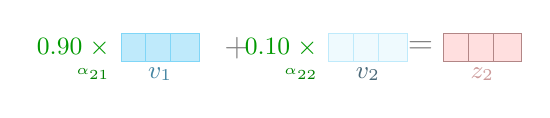
\begin{tikzpicture}[scale=0.88]
    % Layout: coeff [cells] + coeff [cells] = [cells]
    %              v_label           v_label      z_label
    %              alpha             alpha
    % Coefficients left of cells, vector/alpha labels below cells.

    % --- term 1: 0.90 × v1 ---
    \node[font=\small, text=green!60!black, anchor=east] at (0.85, 0) {$0.90\;\times$};
    \foreach \ci in {0,...,2} {
      \pgfmathsetmacro{\cx}{0.90 + \ci*0.36 + 0.18}
      \node[acell, minimum width=0.36cm, minimum height=0.36cm,
            fill=vcol, draw=cyan!50] at (\cx, 0) {};
    }
    \node[font=\small, text=cyan!60!black] at (1.44, -0.38) {$v_1$};
    \node[font=\tiny, text=green!50!black, anchor=east] at (0.85, -0.38) {$\alpha_{21}$};

    % --- + ---
    \node[font=\large, gray] at (2.55, 0) {$+$};

    % --- term 2: 0.10 × v2 ---
    \node[font=\small, text=green!60!black, anchor=east] at (3.85, 0) {$0.10\;\times$};
    \foreach \ci in {0,...,2} {
      \pgfmathsetmacro{\cx}{3.90 + \ci*0.36 + 0.18}
      \node[acell, minimum width=0.36cm, minimum height=0.36cm,
            fill=vcol!25, draw=cyan!25] at (\cx, 0) {};
    }
    \node[font=\small, text=cyan!40!black] at (4.44, -0.38) {$v_2$};
    \node[font=\tiny, text=green!50!black, anchor=east] at (3.85, -0.38) {$\alpha_{22}$};

    % --- = ---
    \node[font=\large, gray] at (5.20, 0) {$=$};

    % --- z2 output ---
    \foreach \ci in {0,...,2} {
      \pgfmathsetmacro{\cx}{5.55 + \ci*0.36 + 0.18}
      \node[acell, minimum width=0.36cm, minimum height=0.36cm,
            fill=zcol, draw=pink!70!black] at (\cx, 0) {};
    }
    \node[font=\small\bfseries, text=pink!80!black] at (6.09, -0.38) {$z_2$};
  \end{tikzpicture}
  \end{center}
\end{frame}

% -----------------------------------------------------------------------
\begin{frame}{Self-Attention: Matrix Form}
  \begin{itemize}
    \item Stack all tokens row-wise into $X \in \mathbb{R}^{T \times d}$.
    \item All queries, keys, and values are computed in \textbf{one matrix multiply}.
  \end{itemize}

  \begin{center}
  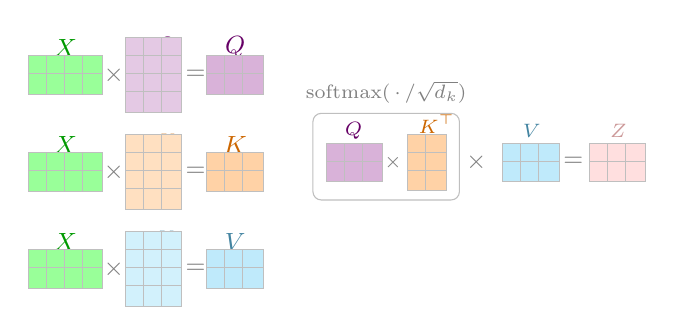
\begin{tikzpicture}[scale=0.88]
    % T=2, d=4, dk=3.  Cell size c=0.26.
    % Left side: three rows  X × W = Q / K / V
    % Positions computed so × and = are centred in their gaps.
    %   X:  x 0.00–1.04      centre 0.52
    %   ×:  x 1.22
    %   W:  x 1.40–2.18      centre 1.79
    %   =:  x 2.40
    %   R:  x 2.58–3.36      centre 2.97

    % === Row 1: Q ===
    \node[font=\small\bfseries, text=green!60!black]  at (0.52, 3.65) {$X$};
    \node[font=\small\bfseries, text=violet!80!black] at (1.79, 3.65) {$W^Q$};
    \node[font=\small\bfseries, text=violet!80!black] at (2.97, 3.65) {$Q$};
    \foreach \ri in {0,...,1} {
      \foreach \ci in {0,...,3} {
        \pgfmathsetmacro{\cx}{0.00 + \ci*0.26 + 0.13}
        \pgfmathsetmacro{\cy}{3.26 - \ri*0.26 + 0.13}
        \node[acell, fill=xcol] at (\cx, \cy) {};
      }
    }
    \node[font=\small, gray] at (1.22, 3.26) {$\times$};
    \foreach \ri in {0,...,3} {
      \foreach \ci in {0,...,2} {
        \pgfmathsetmacro{\cx}{1.40 + \ci*0.26 + 0.13}
        \pgfmathsetmacro{\cy}{3.26 + 0.26 - \ri*0.26 + 0.13}
        \node[acell, fill=qcol!70] at (\cx, \cy) {};
      }
    }
    \node[font=\small, gray] at (2.40, 3.26) {$=$};
    \foreach \ri in {0,...,1} {
      \foreach \ci in {0,...,2} {
        \pgfmathsetmacro{\cx}{2.58 + \ci*0.26 + 0.13}
        \pgfmathsetmacro{\cy}{3.26 - \ri*0.26 + 0.13}
        \node[acell, fill=qcol] at (\cx, \cy) {};
      }
    }

    % === Row 2: K ===
    \node[font=\small\bfseries, text=green!60!black]  at (0.52, 2.25) {$X$};
    \node[font=\small\bfseries, text=orange!80!black] at (1.79, 2.25) {$W^K$};
    \node[font=\small\bfseries, text=orange!80!black] at (2.97, 2.25) {$K$};
    \foreach \ri in {0,...,1} {
      \foreach \ci in {0,...,3} {
        \pgfmathsetmacro{\cx}{0.00 + \ci*0.26 + 0.13}
        \pgfmathsetmacro{\cy}{1.86 - \ri*0.26 + 0.13}
        \node[acell, fill=xcol] at (\cx, \cy) {};
      }
    }
    \node[font=\small, gray] at (1.22, 1.86) {$\times$};
    \foreach \ri in {0,...,3} {
      \foreach \ci in {0,...,2} {
        \pgfmathsetmacro{\cx}{1.40 + \ci*0.26 + 0.13}
        \pgfmathsetmacro{\cy}{1.86 + 0.26 - \ri*0.26 + 0.13}
        \node[acell, fill=kcol!70] at (\cx, \cy) {};
      }
    }
    \node[font=\small, gray] at (2.40, 1.86) {$=$};
    \foreach \ri in {0,...,1} {
      \foreach \ci in {0,...,2} {
        \pgfmathsetmacro{\cx}{2.58 + \ci*0.26 + 0.13}
        \pgfmathsetmacro{\cy}{1.86 - \ri*0.26 + 0.13}
        \node[acell, fill=kcol] at (\cx, \cy) {};
      }
    }

    % === Row 3: V ===
    \node[font=\small\bfseries, text=green!60!black] at (0.52, 0.85) {$X$};
    \node[font=\small\bfseries, text=cyan!60!black]  at (1.79, 0.85) {$W^V$};
    \node[font=\small\bfseries, text=cyan!60!black]  at (2.97, 0.85) {$V$};
    \foreach \ri in {0,...,1} {
      \foreach \ci in {0,...,3} {
        \pgfmathsetmacro{\cx}{0.00 + \ci*0.26 + 0.13}
        \pgfmathsetmacro{\cy}{0.46 - \ri*0.26 + 0.13}
        \node[acell, fill=xcol] at (\cx, \cy) {};
      }
    }
    \node[font=\small, gray] at (1.22, 0.46) {$\times$};
    \foreach \ri in {0,...,3} {
      \foreach \ci in {0,...,2} {
        \pgfmathsetmacro{\cx}{1.40 + \ci*0.26 + 0.13}
        \pgfmathsetmacro{\cy}{0.46 + 0.26 - \ri*0.26 + 0.13}
        \node[acell, fill=vcol!70] at (\cx, \cy) {};
      }
    }
    \node[font=\small, gray] at (2.40, 0.46) {$=$};
    \foreach \ri in {0,...,1} {
      \foreach \ci in {0,...,2} {
        \pgfmathsetmacro{\cx}{2.58 + \ci*0.26 + 0.13}
        \pgfmathsetmacro{\cy}{0.46 - \ri*0.26 + 0.13}
        \node[acell, fill=vcol] at (\cx, \cy) {};
      }
    }

    % === Right side: softmax(QK^T / √dk) · V = Z ===
    % Single illustration with softmax box wrapping Q × K^T / √dk
    \def\cs{0.26}
    \def\ry{2.00}  % vertical centre

    % Q block (T=2, dk=3)
    \node[font=\scriptsize\bfseries, text=violet!80!black]
      at (4.68, \ry+0.45) {$Q$};
    \foreach \ri in {0,...,1} {
      \foreach \ci in {0,...,2} {
        \pgfmathsetmacro{\cx}{4.30 + \ci*\cs + \cs/2}
        \pgfmathsetmacro{\cy}{\ry - \ri*\cs + \cs/2}
        \node[acell, fill=qcol] at (\cx, \cy) {};
      }
    }

    % × between Q and K^T
    \node[font=\scriptsize, gray] at (5.25, \ry) {$\times$};

    % K^T block (dk=3, T=2)
    \node[font=\scriptsize\bfseries, text=orange!80!black]
      at (5.88, \ry+0.55) {$K^\top$};
    \foreach \ri in {0,...,2} {
      \foreach \ci in {0,...,1} {
        \pgfmathsetmacro{\cx}{5.48 + \ci*\cs + \cs/2}
        \pgfmathsetmacro{\cy}{\ry + \cs/2 - \ri*\cs + \cs/2}
        \node[acell, fill=kcol] at (\cx, \cy) {};
      }
    }

    % Softmax box tightly around Q × K^T only
    % Q spans x 4.30–5.08, K^T spans x 5.48–6.00, y range ≈ ry-0.26 to ry+0.52
    \node[draw=gray!50, rounded corners=3pt, fill=none,
          minimum width=1.86cm, minimum height=1.10cm,
          label={[font=\scriptsize, gray]above:$\mathrm{softmax}(\,\cdot\, / \sqrt{d_k})$}]
      at (5.15, \ry+0.08) {};

    % × outside softmax box (before V)
    \node[font=\small, gray] at (6.45, \ry) {$\times$};

    % V block (T=2, dk=3)
    \node[font=\scriptsize\bfseries, text=cyan!60!black]
      at (7.25, \ry+0.45) {$V$};
    \foreach \ri in {0,...,1} {
      \foreach \ci in {0,...,2} {
        \pgfmathsetmacro{\cx}{6.85 + \ci*\cs + \cs/2}
        \pgfmathsetmacro{\cy}{\ry - \ri*\cs + \cs/2}
        \node[acell, fill=vcol] at (\cx, \cy) {};
      }
    }

    % = sign
    \node[font=\small, gray] at (7.85, \ry) {$=$};

    % Z block (T=2, dk=3)
    \node[font=\scriptsize\bfseries, text=pink!80!black]
      at (8.50, \ry+0.45) {$Z$};
    \foreach \ri in {0,...,1} {
      \foreach \ci in {0,...,2} {
        \pgfmathsetmacro{\cx}{8.10 + \ci*\cs + \cs/2}
        \pgfmathsetmacro{\cy}{\ry - \ri*\cs + \cs/2}
        \node[acell, fill=zcol] at (\cx, \cy) {};
      }
    }

  \end{tikzpicture}
  \end{center}
\end{frame}

\subsection{Multi-Head \& Attention Variants}

% -----------------------------------------------------------------------
\begin{frame}{Multi-Head Attention}
  \begin{itemize}
    \item A single head may miss diverse relationship types.
    \item \textbf{Multi-head attention} runs $h$ heads in parallel, each with its own $W^Q_i, W^K_i, W^V_i$.
  \end{itemize}
  \[
    \mathrm{MHA}(X) = \mathrm{Concat}(z^{(1)}, \ldots, z^{(h)})\, W^O
  \]

  \begin{center}
  \begin{tikzpicture}[scale=0.78,
      head/.style={draw=gray!60, rounded corners=3pt, minimum width=2.6cm,
                   minimum height=0.50cm, font=\small, fill=gray!10},
      arr/.style={-{Stealth[length=3.5pt]}, gray!70}
    ]
    \def\cs{0.22}  % cell size
    % Head y-positions
    \def\yA{3.20}
    \def\yB{1.80}
    \def\yH{0.40}
    \def\yD{1.10}  % dots y

    % ======== 1. DEFINE ALL NODES FIRST ========

    % ---- Input X (T=2, d=4) ----
    \node[font=\small\bfseries, text=green!60!black] at (0.0, 3.70) {$X$};
    \foreach \ri in {0,...,1} {
      \foreach \ci in {0,...,3} {
        \pgfmathsetmacro{\cx}{-0.35 + \ci*\cs + \cs/2}
        \pgfmathsetmacro{\cy}{\yB + \cs/2 - \ri*\cs}
        \node[acell, minimum width=\cs cm, minimum height=\cs cm,
              fill=xcol] at (\cx, \cy) {};
      }
    }
    % Braces for X
    \pgfmathsetmacro{\xRe}{-0.35 + 4*\cs}
    \draw[decorate, decoration={brace, amplitude=2pt, mirror}, gray!50, thin]
      (-0.35-0.04, \yB+\cs) -- (-0.35-0.04, \yB-\cs)
      node[midway, left=3pt, font=\tiny, gray] {$T$};
    \draw[decorate, decoration={brace, amplitude=2pt, mirror}, gray!50, thin]
      (-0.35, \yB-\cs-0.06) -- (\xRe, \yB-\cs-0.06)
      node[midway, below=3pt, font=\tiny, gray] {$d$};

    % ---- Heads ----
    \node[head, fill=violet!15, draw=violet!50, text=violet!80!black]
      (h1) at (3.0, \yA) {Head 1: $W^Q_1, W^K_1, W^V_1$};
    \node[head, fill=violet!10, draw=violet!40, text=violet!70!black]
      (h2) at (3.0, \yB) {Head 2: $W^Q_2, W^K_2, W^V_2$};
    \node[font=\small, gray] at (3.0, \yD) {$\vdots$};
    \node[head, fill=violet!10, draw=violet!40, text=violet!70!black]
      (hh) at (3.0, \yH) {Head $h$: $W^Q_h, W^K_h, W^V_h$};

    % ======== 2. BROADCAST ARROWS (mirror style of z→concat bracket) ========
    % Short horizontal from X right edge, then vertical bar, then arrows to heads
    \draw[gray!70, line width=0.5pt] (0.55, \yB) -- (0.80, \yB);
    \draw[gray!70, line width=0.5pt] (0.80, \yH) -- (0.80, \yA);
    \draw[arr] (0.80, \yA) -- (h1.west);
    \draw[arr] (0.80, \yB) -- (h2.west);
    \draw[arr] (0.80, \yH) -- (hh.west);

    % ======== 3. Z^{(i)} MATRICES (0.80 gap from head right edge) ========
    \def\zx{5.20}  % Z block left x

    % Z^(1)
    \draw[arr] (h1.east) -- (\zx, \yA);
    \node[font=\tiny, text=pink!80!black] at (\zx+0.33, \yA+0.55) {$Z^{(1)}$};
    \foreach \ri in {0,...,1} {
      \foreach \ci in {0,...,2} {
        \pgfmathsetmacro{\cx}{\zx + \ci*\cs + \cs/2}
        \pgfmathsetmacro{\cy}{\yA + \cs/2 - \ri*\cs}
        \node[acell, minimum width=\cs cm, minimum height=\cs cm,
              fill=zcol, draw=pink!70!black] at (\cx, \cy) {};
      }
    }
    % Z^(2)
    \draw[arr] (h2.east) -- (\zx, \yB);
    \node[font=\tiny, text=pink!70!black] at (\zx+0.33, \yB+0.55) {$Z^{(2)}$};
    \foreach \ri in {0,...,1} {
      \foreach \ci in {0,...,2} {
        \pgfmathsetmacro{\cx}{\zx + \ci*\cs + \cs/2}
        \pgfmathsetmacro{\cy}{\yB + \cs/2 - \ri*\cs}
        \node[acell, minimum width=\cs cm, minimum height=\cs cm,
              fill=zcol!60, draw=pink!50] at (\cx, \cy) {};
      }
    }
    % dots
    \node[font=\small, gray] at (\zx+0.33, \yD) {$\vdots$};
    % Z^(h)
    \draw[arr] (hh.east) -- (\zx, \yH);
    \node[font=\tiny, text=pink!70!black] at (\zx+0.33, \yH-0.45) {$Z^{(h)}$};
    \foreach \ri in {0,...,1} {
      \foreach \ci in {0,...,2} {
        \pgfmathsetmacro{\cx}{\zx + \ci*\cs + \cs/2}
        \pgfmathsetmacro{\cy}{\yH + \cs/2 - \ri*\cs}
        \node[acell, minimum width=\cs cm, minimum height=\cs cm,
              fill=zcol!60, draw=pink!50] at (\cx, \cy) {};
      }
    }

    % ======== 4. CONCAT BRACKET ========
    \pgfmathsetmacro{\brkL}{\zx + 3*\cs + 0.10}
    \pgfmathsetmacro{\brkR}{\brkL + 0.30}
    \draw[gray!70, line width=0.5pt] (\brkL, \yA) -- (\brkR, \yA);
    \draw[gray!70, line width=0.5pt] (\brkL, \yB) -- (\brkR, \yB);
    \draw[gray!70, line width=0.5pt] (\brkL, \yH) -- (\brkR, \yH);
    \draw[gray!70, line width=0.5pt] (\brkR, \yH) -- (\brkR, \yA);

    % ======== 5. CONCAT RESULT (T × h·dk) ========
    \pgfmathsetmacro{\catx}{\brkR + 0.30}
    \draw[arr] (\brkR, \yB) -- (\catx, \yB);
    \node[font=\scriptsize, gray] at (\catx+1.0, 2.60) {Concat along $d_k$};
    \node[font=\tiny, gray] at (\catx+1.0, 2.38) {$T\!\times\!h d_k$};
    % Group 1
    \foreach \ri in {0,...,1} {
      \foreach \ci in {0,...,2} {
        \pgfmathsetmacro{\cx}{\catx + \ci*\cs + \cs/2}
        \pgfmathsetmacro{\cy}{\yB + \cs/2 - \ri*\cs}
        \node[acell, minimum width=\cs cm, minimum height=\cs cm,
              fill=zcol, draw=pink!60] at (\cx, \cy) {};
      }
    }
    % Group 2
    \foreach \ri in {0,...,1} {
      \foreach \ci in {0,...,2} {
        \pgfmathsetmacro{\cx}{\catx + 3*\cs + \ci*\cs + \cs/2}
        \pgfmathsetmacro{\cy}{\yB + \cs/2 - \ri*\cs}
        \node[acell, minimum width=\cs cm, minimum height=\cs cm,
              fill=zcol!55, draw=pink!45] at (\cx, \cy) {};
      }
    }
    % dots
    \pgfmathsetmacro{\dotx}{\catx + 6*\cs + 0.30}
    \node[font=\small, gray] at (\dotx, \yB) {$\cdots$};
    % Group h
    \pgfmathsetmacro{\ghx}{\dotx + 0.35}
    \foreach \ri in {0,...,1} {
      \foreach \ci in {0,...,2} {
        \pgfmathsetmacro{\cx}{\ghx + \ci*\cs + \cs/2}
        \pgfmathsetmacro{\cy}{\yB + \cs/2 - \ri*\cs}
        \node[acell, minimum width=\cs cm, minimum height=\cs cm,
              fill=zcol!45, draw=pink!40] at (\cx, \cy) {};
      }
    }

    % ======== 6. W^O (with generous gaps) ========
    \pgfmathsetmacro{\wox}{\ghx + 3*\cs + 1.20}
    \node[draw=gray!60, fill=gray!15, rounded corners=3pt,
          minimum width=0.80cm, minimum height=0.45cm, font=\small]
      (wo) at (\wox, \yB) {$W^O$};
    \pgfmathsetmacro{\woarr}{\ghx + 3*\cs + 0.15}
    \draw[arr] (\woarr, \yB) -- (wo.west);

    % ======== 7. FINAL OUTPUT Z (T×d = 2×4) ========
    \pgfmathsetmacro{\zfx}{\wox + 0.80}
    \draw[arr] (wo.east) -- (\zfx, \yB);
    \node[font=\small\bfseries, text=pink!80!black] at (\zfx+0.44, 3.10) {$Z$};
    \foreach \ri in {0,...,1} {
      \foreach \ci in {0,...,3} {
        \pgfmathsetmacro{\cx}{\zfx + \ci*\cs + \cs/2}
        \pgfmathsetmacro{\cy}{\yB + \cs/2 - \ri*\cs}
        \node[acell, minimum width=\cs cm, minimum height=\cs cm,
              fill=zcol, draw=pink!70!black] at (\cx, \cy) {};
      }
    }
    % Braces for Z
    \pgfmathsetmacro{\zRe}{\zfx + 4*\cs}
    \draw[decorate, decoration={brace, amplitude=2pt}, gray!50, thin]
      (\zRe+0.04, \yB+\cs) -- (\zRe+0.04, \yB-\cs)
      node[midway, right=3pt, font=\tiny, gray] {$T$};
    \draw[decorate, decoration={brace, amplitude=2pt, mirror}, gray!50, thin]
      (\zfx, \yB-\cs-0.06) -- (\zRe, \yB-\cs-0.06)
      node[midway, below=3pt, font=\tiny, gray] {$d$};

  \end{tikzpicture}
  \end{center}

  \begin{itemize}
    \item Each head learns to attend to \emph{different} aspects: syntax, coreference, proximity, \ldots
    \item $W^O \in \mathbb{R}^{hd_k \times d}$ projects the concatenated head outputs back to model dimension $d$.
  \end{itemize}
\end{frame}

% -----------------------------------------------------------------------
\begin{frame}{Causal Self-Attention}
  During \textbf{autoregressive generation}, token $i$ must not attend to future tokens $j > i$.
  We enforce this with an \textbf{upper-triangular mask} applied before softmax.

  \begin{columns}[T]
    \begin{column}{0.50\textwidth}
      \vspace{0.3em}
      \[
        s_{ij} = \begin{cases} q_i^\top k_j / \sqrt{d_k} & j \le i \\ -\infty & j > i \end{cases}
      \]
      After softmax, $-\infty$ becomes $0$, so future positions receive zero weight.

      \vspace{0.5em}
      \begin{alertblock}{Key property}
        Training is fully \textbf{parallel}: the mask ensures valid supervision while all $T$ positions are processed simultaneously.
      \end{alertblock}
    \end{column}
    \begin{column}{0.47\textwidth}
      \begin{center}
      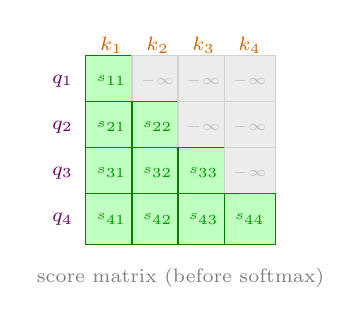
\begin{tikzpicture}[scale=0.90]
        % 4x4 causal mask showing s_{ij} (pre-softmax scores)
        \def\T{4}
        \def\cs{0.65}  % cell size
        \def\ox{0.35}  % x offset
        \def\oy{0.35}  % y offset

        % column labels (keys) above the grid
        \foreach \j in {1,...,4} {
          \pgfmathsetmacro{\lx}{(\j-1)*\cs + \cs/2 + \ox}
          \node[font=\scriptsize, orange!80!black] at (\lx, 4*\cs+\oy+0.18) {$k_{\j}$};
        }
        % row labels (queries) left of the grid
        \foreach \i in {1,...,4} {
          \pgfmathsetmacro{\ly}{(4-\i)*\cs + \cs/2 + \oy}
          \node[font=\scriptsize, violet!80!black, anchor=east] at (\ox-0.08, \ly) {$q_{\i}$};
        }

        % Grid cells
        \foreach \i in {1,...,4} {
          \foreach \j in {1,...,4} {
            \pgfmathsetmacro{\cx}{(\j-1)*\cs + \cs/2 + \ox}
            \pgfmathsetmacro{\cy}{(4-\i)*\cs + \cs/2 + \oy}
            \pgfmathtruncatemacro{\masked}{\j > \i ? 1 : 0}
            \ifnum\masked=1
              % masked (future) -- gray
              \node[minimum width=\cs cm, minimum height=\cs cm,
                    fill=gray!15, draw=gray!35, inner sep=0] at (\cx, \cy) {};
              \node[font=\tiny, gray!50] at (\cx, \cy) {$-\infty$};
            \else
              % allowed (past/present) -- green with s_{ij}
              \node[minimum width=\cs cm, minimum height=\cs cm,
                    fill=green!25, draw=green!50!black, inner sep=0] at (\cx, \cy) {};
              \node[font=\tiny, green!60!black] at (\cx, \cy) {$s_{\i\j}$};
            \fi
          }
        }

        % label
        \node[font=\scriptsize, gray, align=center] at (2*\cs+\ox, -0.15)
          {score matrix (before softmax)};
      \end{tikzpicture}
      \end{center}
    \end{column}
  \end{columns}
\end{frame}

% -----------------------------------------------------------------------
\begin{frame}{Cross-Attention}
  In \textbf{cross-attention}, queries come from one sequence and keys/values from another:
  \begin{itemize}
    \item Allows tokens of one sequence to attend to tokens of another, letting the model align and combine information across two different representations.
    \item \textbf{Decoder} tokens ($T_{\mathrm{dec}}$) produce queries; \textbf{encoder} tokens ($T_{\mathrm{enc}}$) provide keys and values.
    \item The attention weight matrix is $T_{\mathrm{dec}} \times T_{\mathrm{enc}}$ (not square!).
  \end{itemize}

  \begin{center}
  \begin{tikzpicture}[scale=0.75]
    % Source (encoder): T_enc=5, Target (decoder): T_dec=3, d=4, dk=3
    % Layout: Source + Target on top, K/V under Source, Q under Target,
    % Attention matrix to the right, Z below it.
    %
    % Horizontal centres:
    %   Source xsrc=1.8, K xK=0.6, V xV=3.0  (midpoint 1.8 ✓)
    %   Target xtgt=5.8, Q same
    %   Attention matrix xatt=8.8

    \def\cs{0.22}  % cell size

    \def\xsrc{1.80}
    \def\xtgt{5.80}
    \def\xK{0.60}
    \def\xV{3.00}
    \def\xatt{8.80}

    % ======== TOP ROW ========

    % Source X_enc (5 rows × 4 cols)
    \node[font=\small\bfseries, text=green!60!black] at (\xsrc, 5.30)
      {Source ($T_{\mathrm{enc}} \!=\! 5$)};
    \node[font=\scriptsize, text=green!60!black] at (\xsrc, 5.00) {$X_{\mathrm{enc}}$};
    \foreach \ri in {0,...,4} {
      \foreach \ci in {0,...,3} {
        \pgfmathsetmacro{\cx}{\xsrc - 2*\cs + \ci*\cs + \cs/2}
        \pgfmathsetmacro{\cy}{4.50 - \ri*\cs}
        \node[acell, minimum width=\cs cm, minimum height=\cs cm,
              fill=xcol] at (\cx, \cy) {};
      }
    }
    % Brace: rows = T_enc (left side) — top 4.50+cs/2, bottom 4.50-4*cs-cs/2
    \pgfmathsetmacro{\srcL}{\xsrc - 2*\cs}
    \pgfmathsetmacro{\srcTop}{4.50 + \cs/2}
    \pgfmathsetmacro{\srcBot}{4.50 - 4*\cs - \cs/2}
    \draw[decorate, decoration={brace, amplitude=3pt, mirror}, gray!60, thin]
      (\srcL-0.06, \srcTop) -- (\srcL-0.06, \srcBot)
      node[midway, left=4pt, font=\tiny, gray] {$T_{\mathrm{enc}}\!=\!5$};

    % Target X_dec (3 rows × 4 cols)
    \node[font=\small\bfseries, text=violet!70!black] at (\xtgt, 5.30)
      {Target ($T_{\mathrm{dec}} \!=\! 3$)};
    \node[font=\scriptsize, text=violet!70!black] at (\xtgt, 5.00) {$X_{\mathrm{dec}}$};
    \foreach \ri in {0,...,2} {
      \foreach \ci in {0,...,3} {
        \pgfmathsetmacro{\cx}{\xtgt - 2*\cs + \ci*\cs + \cs/2}
        \pgfmathsetmacro{\cy}{4.50 - \ri*\cs}
        \node[acell, minimum width=\cs cm, minimum height=\cs cm,
              fill=qcol!50] at (\cx, \cy) {};
      }
    }
    % Brace: rows = T_dec (right side) — top 4.50+cs/2, bottom 4.50-2*cs-cs/2
    \pgfmathsetmacro{\tgtR}{\xtgt + 2*\cs}
    \pgfmathsetmacro{\tgtTop}{4.50 + \cs/2}
    \pgfmathsetmacro{\tgtBot}{4.50 - 2*\cs - \cs/2}
    \draw[decorate, decoration={brace, amplitude=3pt}, gray!60, thin]
      (\tgtR+0.06, \tgtTop) -- (\tgtR+0.06, \tgtBot)
      node[midway, right=4pt, font=\tiny, gray] {$T_{\mathrm{dec}}\!=\!3$};

    % ======== ARROWS: Source → K,V  and  Target → Q ========
    % Symmetric fan-out from source bottom to matrix centres
    \draw[-{Stealth[length=3pt]}, gray!60, thin]
      (\xsrc-0.20, 3.30) -- node[left, font=\tiny, pos=0.4] {$W^K$} (\xK, 2.55);
    \draw[-{Stealth[length=3pt]}, gray!60, thin]
      (\xsrc+0.20, 3.30) -- node[right, font=\tiny, pos=0.4] {$W^V$} (\xV, 2.55);
    % Vertical from target to Q
    \draw[-{Stealth[length=3pt]}, gray!60, thin]
      (\xtgt, 3.80) -- node[right, font=\tiny, pos=0.4] {$W^Q$} (\xtgt, 2.55);

    % ======== MIDDLE ROW: K, V, Q ========

    % K (5×3), centred at xK — label at top-left corner
    \pgfmathsetmacro{\KLtmp}{\xK - 1.5*\cs}
    \node[font=\scriptsize\bfseries, text=orange!80!black, anchor=south east]
      at (\KLtmp-0.01, 2.40+\cs/2) {$K$};
    \foreach \ri in {0,...,4} {
      \foreach \ci in {0,...,2} {
        \pgfmathsetmacro{\cx}{\xK - 1.5*\cs + \ci*\cs + \cs/2}
        \pgfmathsetmacro{\cy}{2.40 - \ri*\cs}
        \node[acell, minimum width=\cs cm, minimum height=\cs cm,
              fill=kcol] at (\cx, \cy) {};
      }
    }
    % Brace: rows (left side) — top edge 2.40+cs/2, bottom edge 2.40-4*cs-cs/2
    \pgfmathsetmacro{\KL}{\xK - 1.5*\cs}
    \pgfmathsetmacro{\KR}{\xK + 1.5*\cs}
    \pgfmathsetmacro{\Ktop}{2.40 + \cs/2}
    \pgfmathsetmacro{\Kbot}{2.40 - 4*\cs - \cs/2}
    \draw[decorate, decoration={brace, amplitude=2pt, mirror}, gray!50, thin]
      (\KL-0.04, \Ktop) -- (\KL-0.04, \Kbot)
      node[midway, left=3pt, font=\tiny, gray] {$5$};
    % Brace: cols
    \draw[decorate, decoration={brace, amplitude=2pt, mirror}, gray!50, thin]
      (\KL, \Kbot-0.06) -- (\KR, \Kbot-0.06)
      node[midway, below=3pt, font=\tiny, gray] {$d_k$};

    % V (5×3), centred at xV — label at top-left corner
    \pgfmathsetmacro{\VLtmp}{\xV - 1.5*\cs}
    \node[font=\scriptsize\bfseries, text=cyan!60!black, anchor=south east]
      at (\VLtmp-0.01, 2.40+\cs/2) {$V$};
    \foreach \ri in {0,...,4} {
      \foreach \ci in {0,...,2} {
        \pgfmathsetmacro{\cx}{\xV - 1.5*\cs + \ci*\cs + \cs/2}
        \pgfmathsetmacro{\cy}{2.40 - \ri*\cs}
        \node[acell, minimum width=\cs cm, minimum height=\cs cm,
              fill=vcol] at (\cx, \cy) {};
      }
    }
    % Brace: rows (left side)
    \pgfmathsetmacro{\VL}{\xV - 1.5*\cs}
    \pgfmathsetmacro{\VR}{\xV + 1.5*\cs}
    \pgfmathsetmacro{\Vtop}{2.40 + \cs/2}
    \pgfmathsetmacro{\Vbot}{2.40 - 4*\cs - \cs/2}
    \draw[decorate, decoration={brace, amplitude=2pt, mirror}, gray!50, thin]
      (\VL-0.04, \Vtop) -- (\VL-0.04, \Vbot)
      node[midway, left=3pt, font=\tiny, gray] {$5$};

    % Q (3×3), centred at xtgt — label at top-left corner
    \pgfmathsetmacro{\QLtmp}{\xtgt - 1.5*\cs}
    \node[font=\scriptsize\bfseries, text=violet!80!black, anchor=south east]
      at (\QLtmp-0.01, 2.40+\cs/2) {$Q$};
    \foreach \ri in {0,...,2} {
      \foreach \ci in {0,...,2} {
        \pgfmathsetmacro{\cx}{\xtgt - 1.5*\cs + \ci*\cs + \cs/2}
        \pgfmathsetmacro{\cy}{2.40 - \ri*\cs}
        \node[acell, minimum width=\cs cm, minimum height=\cs cm,
              fill=qcol] at (\cx, \cy) {};
      }
    }
    % Brace: rows (left side)
    \pgfmathsetmacro{\QL}{\xtgt - 1.5*\cs}
    \pgfmathsetmacro{\QR}{\xtgt + 1.5*\cs}
    \pgfmathsetmacro{\Qtop}{2.40 + \cs/2}
    \pgfmathsetmacro{\Qbot}{2.40 - 2*\cs - \cs/2}
    \draw[decorate, decoration={brace, amplitude=2pt, mirror}, gray!50, thin]
      (\QL-0.04, \Qtop) -- (\QL-0.04, \Qbot)
      node[midway, left=3pt, font=\tiny, gray] {$3$};
    % Brace: cols
    \draw[decorate, decoration={brace, amplitude=2pt, mirror}, gray!50, thin]
      (\QL, \Qbot-0.06) -- (\QR, \Qbot-0.06)
      node[midway, below=3pt, font=\tiny, gray] {$d_k$};

    % ======== ATTENTION WEIGHT MATRIX (3 × 5) ========
    \node[font=\scriptsize\bfseries, gray] at (\xatt, 3.40) {Attention weights};

    % cells
    \foreach \i in {1,...,3} {
      \foreach \j in {1,...,5} {
        \pgfmathsetmacro{\cx}{\xatt - 2.5*\cs + (\j-1)*\cs + \cs/2}
        \pgfmathsetmacro{\cy}{2.40 - (\i-1)*\cs}
        \pgfmathtruncatemacro{\hilight}{\j == \i ? 1 : 0}
        \ifnum\hilight=1
          \node[acell, minimum width=\cs cm, minimum height=\cs cm,
                fill=green!40, draw=green!50!black] at (\cx, \cy) {};
        \else
          \node[acell, minimum width=\cs cm, minimum height=\cs cm,
                fill=green!12, draw=gray!40] at (\cx, \cy) {};
        \fi
      }
    }
    % Braces — att matrix is 3 rows × 5 cols, top cell at 2.40
    \pgfmathsetmacro{\aR}{\xatt + 2.5*\cs}
    \pgfmathsetmacro{\aL}{\xatt - 2.5*\cs}
    \pgfmathsetmacro{\atop}{2.40 + \cs/2}
    \pgfmathsetmacro{\abot}{2.40 - 2*\cs - \cs/2}
    \draw[decorate, decoration={brace, amplitude=3pt}, gray!50, thin]
      (\aR+0.05, \atop) -- (\aR+0.05, \abot)
      node[midway, right=4pt, font=\tiny, gray] {$T_{\mathrm{dec}}$};
    \draw[decorate, decoration={brace, amplitude=3pt}, gray!50, thin]
      (\aL, \atop+0.06) -- (\aR, \atop+0.06)
      node[midway, above=4pt, font=\tiny, gray] {$T_{\mathrm{enc}}$};

    % ---- Arrows Q,K → attention matrix ----
    \draw[-{Stealth[length=3pt]}, gray!60, thin]
      (\QR+0.10, 2.10) -- (\aL-0.10, 2.10);
    \draw[-{Stealth[length=3pt]}, gray!60, thin]
      (\KR+0.10, 1.90) to[out=-30, in=180] (4.0, 1.10)
      -- (7.2, 1.10) to[out=0, in=-90] (\xatt-0.30, 1.75);

    % ======== OUTPUT Z (3 × dk) — label at top-left corner ========
    \pgfmathsetmacro{\ZLtmp}{\xatt - 1.5*\cs}
    \node[font=\scriptsize\bfseries, text=pink!80!black, anchor=south east]
      at (\ZLtmp-0.01, 0.55+\cs/2) {$Z$};
    \foreach \ri in {0,...,2} {
      \foreach \ci in {0,...,2} {
        \pgfmathsetmacro{\cx}{\xatt - 1.5*\cs + \ci*\cs + \cs/2}
        \pgfmathsetmacro{\cy}{0.55 - \ri*\cs}
        \node[acell, minimum width=\cs cm, minimum height=\cs cm,
              fill=zcol, draw=pink!60] at (\cx, \cy) {};
      }
    }
    % Brace: rows — Z top edge 0.55+cs/2, bottom edge 0.55-2*cs-cs/2
    \pgfmathsetmacro{\Ztop}{0.55 + \cs/2}
    \pgfmathsetmacro{\Zbot}{0.55 - 2*\cs - \cs/2}
    \draw[decorate, decoration={brace, amplitude=2pt, mirror}, gray!50, thin]
      (\xatt - 1.5*\cs - 0.04, \Ztop) -- (\xatt - 1.5*\cs - 0.04, \Zbot)
      node[midway, left=3pt, font=\tiny, gray] {$T_{\mathrm{dec}}$};

    \draw[-{Stealth[length=3pt]}, gray!60, thin]
      (\xatt, 1.70) -- (\xatt, 0.70);

    % formula
    \node[font=\scriptsize, gray] at (\xatt, -0.40)
      {$Z = \mathrm{softmax}\!\bigl(\frac{QK^\top}{\sqrt{d_k}}\bigr) V$};

  \end{tikzpicture}
  \end{center}
\end{frame}

% -----------------------------------------------------------------------
\begin{frame}{Cross-Attention: Machine Translation Example}
  \begin{itemize}
    \item \textbf{Encoder} processes the source sentence (French) into key/value representations.
    \item \textbf{Decoder} generates the target sentence (English) one token at a time, using cross-attention to query the encoder output.
    \item Line thickness shows attention weight: each decoder token focuses on the most relevant source token.
  \end{itemize}

  \begin{center}
  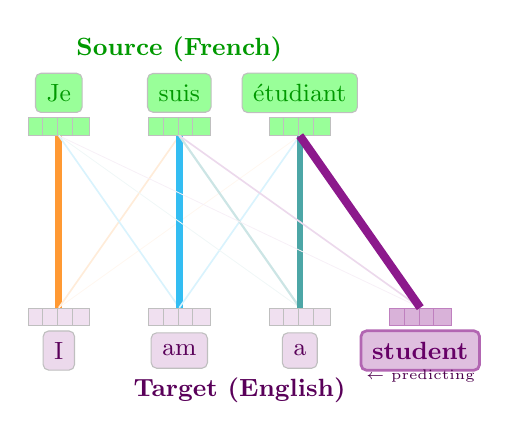
\begin{tikzpicture}[scale=0.85,
      tok/.style={draw=gray!50, rounded corners=2pt, minimum height=0.45cm,
                  inner sep=4pt, font=\small},
    ]
    \def\gap{1.80}

    % ======== ENCODER (source, top) ========
    % "Je suis étudiant" (3 tokens)
    \node[font=\small\bfseries, text=green!60!black] at (1*\gap, 4.50)
      {Source (French)};
    \foreach \j/\tok in {0/Je, 1/suis, 2/\'{e}tudiant} {
      \pgfmathsetmacro{\sx}{\j * \gap}
      \node[tok, fill=xcol, text=green!60!black] (src\j) at (\sx, 3.85) {\tok};
      \foreach \ci in {0,...,3} {
        \pgfmathsetmacro{\cx}{\sx - 2*0.22 + \ci*0.22 + 0.11}
        \node[acell, minimum width=0.22cm, minimum height=0.22cm,
              fill=xcol] at (\cx, 3.35) {};
      }
    }

    % ======== DECODER (target, bottom) ========
    % "I am a student" (4 tokens)
    \node[font=\small\bfseries, text=violet!70!black] at (1.5*\gap, -0.60)
      {Target (English)};

    % Already generated tokens
    \foreach \i/\tok in {0/I, 1/am, 2/a} {
      \pgfmathsetmacro{\tx}{\i * \gap}
      \node[tok, fill=qcol!50, text=violet!70!black] (tgt\i) at (\tx, 0) {\tok};
      \foreach \ci in {0,...,3} {
        \pgfmathsetmacro{\cx}{\tx - 2*0.22 + \ci*0.22 + 0.11}
        \node[acell, minimum width=0.22cm, minimum height=0.22cm,
              fill=qcol!40] at (\cx, 0.50) {};
      }
    }

    % Currently generating token (highlighted)
    \pgfmathsetmacro{\curtx}{3 * \gap}
    \node[tok, fill=violet!25, draw=violet!60, line width=1pt,
          text=violet!80!black, font=\small\bfseries]
      (tgt3) at (\curtx, 0) {student};
    \node[font=\tiny, text=violet!60!black] at (\curtx, -0.38) {$\leftarrow$ predicting};
    \foreach \ci in {0,...,3} {
      \pgfmathsetmacro{\cx}{\curtx - 2*0.22 + \ci*0.22 + 0.11}
      \node[acell, minimum width=0.22cm, minimum height=0.22cm,
            fill=qcol, draw=violet!50] at (\cx, 0.50) {};
    }

    % ======== ATTENTION CONNECTIONS ========
    % Lines from each target token to source tokens, opacity ∝ weight

    % --- "I" (tgt0) attention ---
    % Je=0.85, suis=0.10, étudiant=0.05
    \draw[orange!80, line width=2.5pt]   (0, 3.21) -- (0, 0.64);
    \draw[orange!15, line width=0.6pt]   (1*\gap, 3.21) -- (0, 0.64);
    \draw[orange!6, line width=0.3pt]    (2*\gap, 3.21) -- (0, 0.64);

    % --- "am" (tgt1) attention ---
    % Je=0.10, suis=0.80, étudiant=0.10
    \draw[cyan!15, line width=0.6pt]     (0, 3.21) -- (1*\gap, 0.64);
    \draw[cyan!80, line width=2.5pt]     (1*\gap, 3.21) -- (1*\gap, 0.64);
    \draw[cyan!15, line width=0.6pt]     (2*\gap, 3.21) -- (1*\gap, 0.64);

    % --- "a" (tgt2) attention ---
    % Je=0.05, suis=0.15, étudiant=0.80
    \draw[teal!6, line width=0.3pt]      (0, 3.21) -- (2*\gap, 0.64);
    \draw[teal!20, line width=0.8pt]     (1*\gap, 3.21) -- (2*\gap, 0.64);
    \draw[teal!70, line width=2.0pt]     (2*\gap, 3.21) -- (2*\gap, 0.64);

    % --- "student" (tgt3, currently generating) attention ---
    % Je=0.02, suis=0.08, étudiant=0.90
    \draw[violet!6, line width=0.3pt]    (0, 3.21) -- (\curtx, 0.64);
    \draw[violet!15, line width=0.6pt]   (1*\gap, 3.21) -- (\curtx, 0.64);
    \draw[violet!90, line width=3.0pt]   (2*\gap, 3.21) -- (\curtx, 0.64);

  \end{tikzpicture}
  \end{center}
\end{frame}

\subsection{Transformer Architecture}

% -----------------------------------------------------------------------
\begin{frame}{Transformer Architecture: Encoder \& Decoder}
  A transformer consists of an \textbf{encoder} and a \textbf{decoder}, each built from a stack of identical blocks.

  \begin{center}
  \begin{tikzpicture}[scale=0.88,
      encblock/.style={draw=green!60!black, fill=green!15, rounded corners=3pt,
                       minimum width=2.8cm, minimum height=0.52cm, font=\small,
                       text=green!50!black},
      decblock/.style={draw=magenta!50!black, fill=magenta!12, rounded corners=3pt,
                       minimum width=2.8cm, minimum height=0.52cm, font=\small,
                       text=magenta!50!black},
      tok/.style={draw=gray!50, rounded corners=2pt, minimum height=0.38cm,
                  inner sep=3pt, font=\small\strut},
      arr/.style={-{Stealth[length=3pt]}, gray!50, thin},
      xarr/.style={-{Stealth[length=3pt]}, green!50!black, thin},
    ]
    \def\encX{-2.4}
    \def\decX{2.4}
    \def\gap{0.78}

    % ---- Encoder stack ----
    \foreach \i in {0,...,5} {
      \pgfmathsetmacro{\y}{\i*\gap}
      \node[encblock] (enc\i) at (\encX, \y) {ENCODER};
    }
    % ---- Decoder stack ----
    \foreach \i in {0,...,5} {
      \pgfmathsetmacro{\y}{\i*\gap}
      \node[decblock] (dec\i) at (\decX, \y) {DECODER};
    }
    % ---- Arrows within encoder stack ----
    \foreach \i in {0,...,4} {
      \pgfmathtruncatemacro{\j}{\i+1}
      \draw[arr] (enc\i.north) -- (enc\j.south);
    }
    % ---- Arrows within decoder stack ----
    \foreach \i in {0,...,4} {
      \pgfmathtruncatemacro{\j}{\i+1}
      \draw[arr] (dec\i.north) -- (dec\j.south);
    }
    % ---- Cross-attention arrows: top encoder -> each decoder ----
    \foreach \i in {0,...,5} {
      \draw[xarr] (enc5.east) -- (dec\i.west);
    }
    % ---- Input tokens ----
    \node[tok, fill=green!12] (in1) at (\encX-1.1, -1.0) {\textit{je}};
    \node[tok, fill=green!12] (in2) at (\encX,     -1.0) {\textit{suis}};
    \node[tok, fill=green!12] (in3) at (\encX+1.1, -1.0) {\textit{\'{e}tudiant}};
    \node[font=\small\bfseries, gray, anchor=east] at ([xshift=-0.2cm]in1.south west) {INPUT:};
    \draw[arr] (in2.north) -- (enc0.south);
    % ---- Output tokens ----
    \pgfmathsetmacro{\topY}{5*\gap + 0.95}
    \node[tok, fill=magenta!10] (out1) at (\decX-1.35, \topY) {\textit{I}};
    \node[tok, fill=magenta!10] (out2) at (\decX-0.45, \topY) {\textit{am}};
    \node[tok, fill=magenta!10] (out3) at (\decX+0.45, \topY) {\textit{a}};
    \node[tok, fill=magenta!10] (out4) at (\decX+1.50, \topY) {\textit{student}};
    \node[font=\small\bfseries, gray, anchor=east] at ([xshift=-0.2cm]out1.north west) {OUTPUT:};
    \draw[arr] (dec5.north) -- (out2.south -| dec5.north);
    % ---- Surrounding boxes ----
    \begin{scope}[on background layer]
      \node[draw=green!40, fill=green!4, rounded corners=6pt,
            fit=(enc0)(enc5), inner xsep=10pt, inner ysep=8pt] {};
      \node[draw=magenta!35, fill=magenta!3, rounded corners=6pt,
            fit=(dec0)(dec5), inner xsep=10pt, inner ysep=8pt] {};
    \end{scope}
  \end{tikzpicture}
  \end{center}

  \begin{itemize}
    \item \textbf{Encoder}: processes the full input sequence into feature vectors
    \item \textbf{Decoder}: generates output tokens one at a time, conditioned on encoder features and past outputs
  \end{itemize}
\end{frame}

% -----------------------------------------------------------------------
\begin{frame}{Encoder Block}
  Each encoder block has two sub-layers, each wrapped with a residual connection and layer normalization:
  \begin{enumerate}
    \item \textbf{Self-Attention}: exchanges information between tokens (mixing)
    \item \textbf{Feed-Forward MLP}: per-token nonlinear transformation (no mixing)
  \end{enumerate}

  \begin{columns}[T]
    \begin{column}{0.38\textwidth}
      \vspace{0.8em}
      \textbf{Sub-layer 1} (attention):
      \begin{align*}
        Z &= \mathrm{MHA}(X) \\
        X' &= \mathrm{LayerNorm}(X + Z)
      \end{align*}

      \vspace{0.3em}
      \textbf{Sub-layer 2} (feed-forward):
      \begin{align*}
        F &= \mathrm{FFN}(X') \\
          &= \underbrace{W_2}_{d \times d_{\mathrm{ff}}}\,\mathrm{GELU}\!\bigl(\underbrace{W_1}_{d_{\mathrm{ff}} \times d}\, X'\bigr) \\
        R &= \mathrm{LayerNorm}(X' + F)
      \end{align*}

      \begin{itemize}
        \item {\small $d_{\mathrm{ff}} = 4d$ (expand then contract).}
      \end{itemize}
    \end{column}
    \begin{column}{0.60\textwidth}
      \begin{center}
      \begin{tikzpicture}[scale=0.72,
          block/.style={draw=gray!60, rounded corners=5pt, minimum height=0.60cm,
                        inner sep=5pt, font=\small},
          arr/.style={-{Stealth[length=4pt]}, gray!70, thick},
        ]
        \def\cs{0.20}
        \def\xA{-1.40}
        \def\xB{1.40}

        % ======== INPUT TOKENS ========
        \node[font=\small\bfseries, text=green!60!black] at (\xA, -0.40) {\textit{Thinking}};
        \node[font=\small\bfseries, text=green!60!black] at (\xB, -0.40) {\textit{Machines}};

        \node[font=\tiny, text=green!60!black, anchor=east] at (\xA-0.30, 0.10) {$x_1$};
        \foreach \ci in {0,...,3} {
          \pgfmathsetmacro{\cx}{\xA - 2*\cs + \ci*\cs + \cs/2}
          \node[acell, minimum width=\cs cm, minimum height=\cs cm,
                fill=xcol] at (\cx, 0.10) {};
        }
        \node[font=\tiny, text=green!60!black, anchor=east] at (\xB-0.30, 0.10) {$x_2$};
        \foreach \ci in {0,...,3} {
          \pgfmathsetmacro{\cx}{\xB - 2*\cs + \ci*\cs + \cs/2}
          \node[acell, minimum width=\cs cm, minimum height=\cs cm,
                fill=xcol] at (\cx, 0.10) {};
        }

        \draw[arr] (\xA, 0.30) -- (\xA, 0.75);
        \draw[arr] (\xB, 0.30) -- (\xB, 0.75);

        % ======== SELF-ATTENTION ========
        \node[block, fill=orange!12, draw=orange!40,
              minimum width=4.8cm, text=orange!80!black]
          (sa) at (0, 1.05) {Self-Attention};

        \draw[arr] (\xA, 1.38) -- (\xA, 2.45);
        \draw[arr] (\xB, 1.38) -- (\xB, 2.45);

        % ======== ADD & NORM 1 ========
        \node[block, fill=yellow!15, draw=yellow!50!black,
              minimum width=4.8cm, font=\small, text=yellow!50!black]
          (an1) at (0, 2.75) {Add \& LayerNorm};

        % Residual 1
        \draw[gray!50, thin, dashed, rounded corners=3pt]
          (\xA, 0.55) -- (-3.70, 0.55) -- (-3.70, 2.75) -- (an1.west);
        \draw[gray!50, thin, dashed, rounded corners=3pt]
          (\xB, 0.55) -- (3.70, 0.55) -- (3.70, 2.75) -- (an1.east);

        \draw[arr] (\xA, 3.05) -- (\xA, 3.80);
        \draw[arr] (\xB, 3.05) -- (\xB, 3.80);

        % ======== FEED-FORWARD ========
        \node[block, fill=cyan!12, draw=cyan!40,
              minimum width=1.8cm, text=cyan!60!black]
          (ff1) at (\xA, 4.10) {Feed-Forward};
        \node[block, fill=cyan!12, draw=cyan!40,
              minimum width=1.8cm, text=cyan!60!black]
          (ff2) at (\xB, 4.10) {Feed-Forward};

        \draw[arr] (\xA, 4.43) -- (\xA, 5.15);
        \draw[arr] (\xB, 4.43) -- (\xB, 5.15);

        % ======== ADD & NORM 2 ========
        \node[block, fill=yellow!15, draw=yellow!50!black,
              minimum width=4.8cm, font=\small, text=yellow!50!black]
          (an2) at (0, 5.45) {Add \& LayerNorm};

        % Residual 2
        \draw[gray!50, thin, dashed, rounded corners=3pt]
          (\xA, 3.40) -- (-3.70, 3.40) -- (-3.70, 5.45) -- (an2.west);
        \draw[gray!50, thin, dashed, rounded corners=3pt]
          (\xB, 3.40) -- (3.70, 3.40) -- (3.70, 5.45) -- (an2.east);

        % Output
        \draw[arr] (\xA, 5.75) -- (\xA, 6.10);
        \draw[arr] (\xB, 5.75) -- (\xB, 6.10);

        \node[font=\tiny, text=blue!60!black, anchor=east] at (\xA-0.30, 6.30) {$r_1$};
        \foreach \ci in {0,...,3} {
          \pgfmathsetmacro{\cx}{\xA - 2*\cs + \ci*\cs + \cs/2}
          \node[acell, minimum width=\cs cm, minimum height=\cs cm,
                fill=blue!20, draw=blue!40] at (\cx, 6.30) {};
        }
        \node[font=\tiny, text=blue!60!black, anchor=east] at (\xB-0.30, 6.30) {$r_2$};
        \foreach \ci in {0,...,3} {
          \pgfmathsetmacro{\cx}{\xB - 2*\cs + \ci*\cs + \cs/2}
          \node[acell, minimum width=\cs cm, minimum height=\cs cm,
                fill=blue!20, draw=blue!40] at (\cx, 6.30) {};
        }

        % ======== BORDER ========
        \draw[green!40!black, rounded corners=8pt, line width=1pt]
          (-4.00, 0.40) rectangle (4.00, 6.05);
        \node[font=\small\bfseries, text=green!40!black]
          at (0, 6.65) {Encoder Block};

      \end{tikzpicture}
      \end{center}
      \vspace{-0.3em}
      \begin{itemize}
        \item {\small Dashed lines \tikz[baseline=-0.5ex]{\draw[gray!50, thin, dashed] (0,0) -- (0.6,0);} = residual connections.}
      \end{itemize}
    \end{column}
  \end{columns}
\end{frame}

% -----------------------------------------------------------------------
\begin{frame}{Decoder Block}
  Each decoder block has \textbf{three} sub-layers (encoder--decoder model) or two (decoder-only):
  \begin{enumerate}
    \item \textbf{Causal Self-Attention}: tokens attend only to past positions
    \item \textbf{Cross-Attention}: queries from decoder, keys/values from encoder (omitted in decoder-only)
    \item \textbf{Feed-Forward MLP}: per-token nonlinear transformation
  \end{enumerate}

  \begin{columns}[T]
    \begin{column}{0.38\textwidth}
      \vspace{0.5em}
      \textbf{Sub-layer 1} (causal attention):
      \begin{align*}
        Z &= \mathrm{CausalMHA}(Y) \\
        Y' &= \mathrm{LN}(Y + Z)
      \end{align*}

      \textbf{Sub-layer 2} (cross-attention):
      \begin{align*}
        C &= \mathrm{CrossMHA}(Y', R) \\
        Y'' &= \mathrm{LN}(Y' + C)
      \end{align*}

      \textbf{Sub-layer 3} (feed-forward):
      \begin{align*}
        F &= \mathrm{FFN}(Y'') \\
        O &= \mathrm{LN}(Y'' + F)
      \end{align*}

      \begin{itemize}
        \item {\small $R$ = encoder output.}
      \end{itemize}
    \end{column}
    \begin{column}{0.60\textwidth}
      \begin{center}
      \begin{tikzpicture}[scale=0.46,
          block/.style={draw=gray!60, rounded corners=5pt, minimum height=0.55cm,
                        inner sep=3pt, font=\footnotesize},
          arr/.style={-{Stealth[length=4pt]}, gray!70, thick},
        ]
        \def\cs{0.20}
        \def\xA{-2.10}
        \def\xB{2.10}

        % Block centers (uniform vertical spacing of 1.65)
        \def\ycsa{1.30}
        \def\yana{2.95}
        \def\yca{4.60}
        \def\yanb{6.25}
        \def\yff{7.90}
        \def\yanc{9.55}

        % ======== INPUT TOKENS (outside the outer block) ========
        \node[font=\small\bfseries, text=violet!70!black] at (\xA, -0.80) {\textit{tok$_1$}};
        \node[font=\small\bfseries, text=violet!70!black] at (\xB, -0.80) {\textit{tok$_2$}};

        \node[font=\tiny, text=violet!70!black, anchor=east] at (\xA-0.30, -0.20) {$y_1$};
        \foreach \ci in {0,...,3} {
          \pgfmathsetmacro{\cx}{\xA - 2*\cs + \ci*\cs + \cs/2}
          \node[acell, minimum width=\cs cm, minimum height=\cs cm,
                fill=qcol!50] at (\cx, -0.20) {};
        }
        \node[font=\tiny, text=violet!70!black, anchor=east] at (\xB-0.30, -0.20) {$y_2$};
        \foreach \ci in {0,...,3} {
          \pgfmathsetmacro{\cx}{\xB - 2*\cs + \ci*\cs + \cs/2}
          \node[acell, minimum width=\cs cm, minimum height=\cs cm,
                fill=qcol!50] at (\cx, -0.20) {};
        }

        % ======== CAUSAL SELF-ATTENTION ========
        \node[block, fill=orange!12, draw=orange!40,
              minimum width=4.8cm, text=orange!80!black]
          (csa) at (0, \ycsa) {Causal Self-Attention};

        \draw[arr] let \p1=(csa.south) in (\xA, 0.05) -- (\xA, \y1);
        \draw[arr] let \p1=(csa.south) in (\xB, 0.05) -- (\xB, \y1);

        % ======== ADD & NORM 1 ========
        \node[block, fill=yellow!15, draw=yellow!50!black,
              minimum width=4.8cm, font=\footnotesize, text=yellow!50!black]
          (an1) at (0, \yana) {Add \& LN};

        \draw[arr] let \p1=(csa.north),\p2=(an1.south) in (\xA, \y1) -- (\xA, \y2);
        \draw[arr] let \p1=(csa.north),\p2=(an1.south) in (\xB, \y1) -- (\xB, \y2);

        % Residual 1 (around causal self-attention)
        \draw[gray!50, thin, dashed, rounded corners=3pt]
          (\xA, 0.55) -- (-5.65, 0.55) -- (-5.65, \yana) -- (an1.west);
        \draw[gray!50, thin, dashed, rounded corners=3pt]
          (\xB, 0.55) -- (5.65, 0.55) -- (5.65, \yana) -- (an1.east);

        % ======== CROSS-ATTENTION ========
        \node[block, fill=green!10, draw=green!40!black,
              minimum width=4.8cm, text=green!50!black]
          (ca) at (0, \yca) {Cross-Attention};

        \draw[arr] let \p1=(an1.north),\p2=(ca.south) in (\xA, \y1) -- (\xA, \y2);
        \draw[arr] let \p1=(an1.north),\p2=(ca.south) in (\xB, \y1) -- (\xB, \y2);

        % Encoder input arrow from the left (outside the new wider border)
        \node[font=\tiny, text=green!60!black, anchor=east] at (-6.10, \yca)
          {$K,V$ from encoder $\rightarrow$};
        \draw[arr, green!50!black] (-5.95, \yca) -- (ca.west);

        % ======== ADD & NORM 2 ========
        \node[block, fill=yellow!15, draw=yellow!50!black,
              minimum width=4.8cm, font=\footnotesize, text=yellow!50!black]
          (an2) at (0, \yanb) {Add \& LN};

        \draw[arr] let \p1=(ca.north),\p2=(an2.south) in (\xA, \y1) -- (\xA, \y2);
        \draw[arr] let \p1=(ca.north),\p2=(an2.south) in (\xB, \y1) -- (\xB, \y2);

        % Residual 2 (around cross-attention)
        \draw[gray!50, thin, dashed, rounded corners=3pt]
          (\xA, 3.78) -- (-5.65, 3.78) -- (-5.65, \yanb) -- (an2.west);
        \draw[gray!50, thin, dashed, rounded corners=3pt]
          (\xB, 3.78) -- (5.65, 3.78) -- (5.65, \yanb) -- (an2.east);

        % ======== FEED-FORWARD ========
        \node[block, fill=cyan!12, draw=cyan!40,
              minimum width=1.8cm, text=cyan!60!black]
          (ff1) at (\xA, \yff) {Feed-Forward};
        \node[block, fill=cyan!12, draw=cyan!40,
              minimum width=1.8cm, text=cyan!60!black]
          (ff2) at (\xB, \yff) {Feed-Forward};

        \draw[arr] let \p1=(an2.north),\p2=(ff1.south) in (\xA, \y1) -- (\xA, \y2);
        \draw[arr] let \p1=(an2.north),\p2=(ff2.south) in (\xB, \y1) -- (\xB, \y2);

        % ======== ADD & NORM 3 ========
        \node[block, fill=yellow!15, draw=yellow!50!black,
              minimum width=4.8cm, font=\footnotesize, text=yellow!50!black]
          (an3) at (0, \yanc) {Add \& LN};

        \draw[arr] let \p1=(ff1.north),\p2=(an3.south) in (\xA, \y1) -- (\xA, \y2);
        \draw[arr] let \p1=(ff2.north),\p2=(an3.south) in (\xB, \y1) -- (\xB, \y2);

        % Residual 3 (around feed-forward)
        \draw[gray!50, thin, dashed, rounded corners=3pt]
          (\xA, 7.08) -- (-5.65, 7.08) -- (-5.65, \yanc) -- (an3.west);
        \draw[gray!50, thin, dashed, rounded corners=3pt]
          (\xB, 7.08) -- (5.65, 7.08) -- (5.65, \yanc) -- (an3.east);

        % Output (cells outside the outer block)
        \draw[arr] let \p1=(an3.north) in (\xA, \y1) -- (\xA, 10.48);
        \draw[arr] let \p1=(an3.north) in (\xB, \y1) -- (\xB, 10.48);

        \node[font=\tiny, text=blue!60!black, anchor=east] at (\xA-0.30, 10.70) {$o_1$};
        \foreach \ci in {0,...,3} {
          \pgfmathsetmacro{\cx}{\xA - 2*\cs + \ci*\cs + \cs/2}
          \node[acell, minimum width=\cs cm, minimum height=\cs cm,
                fill=blue!20, draw=blue!40] at (\cx, 10.70) {};
        }
        \node[font=\tiny, text=blue!60!black, anchor=east] at (\xB-0.30, 10.70) {$o_2$};
        \foreach \ci in {0,...,3} {
          \pgfmathsetmacro{\cx}{\xB - 2*\cs + \ci*\cs + \cs/2}
          \node[acell, minimum width=\cs cm, minimum height=\cs cm,
                fill=blue!20, draw=blue!40] at (\cx, 10.70) {};
        }

        % ======== BORDER (wider, encloses residuals; input/output cells now outside) ========
        \draw[violet!40!black, rounded corners=8pt, line width=1pt]
          (-6.00, 0.40) rectangle (6.00, 10.30);
        \node[font=\small\bfseries, text=violet!40!black]
          at (0, 11.55) {Decoder Block};

      \end{tikzpicture}
      \end{center}
      \vspace{-0.3em}
      \begin{itemize}
        \item {\small Dashed lines \tikz[baseline=-0.5ex]{\draw[gray!50, thin, dashed] (0,0) -- (0.6,0);} = residual connections.}
      \end{itemize}
    \end{column}
  \end{columns}
\end{frame}

\subsection{Positional Encoding}

% -----------------------------------------------------------------------
\begin{frame}{Positional Encoding}
  Self-attention is \textbf{permutation equivariant}: it has no notion of token order.
  We add a \textbf{positional encoding} to each embedding to inject position information.

  \begin{center}
  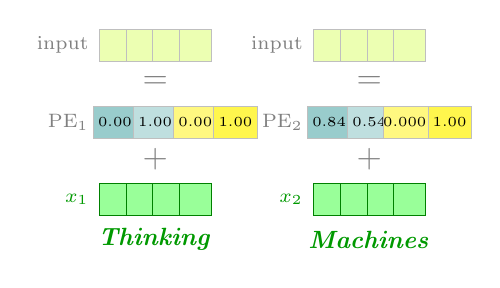
\begin{tikzpicture}[scale=0.85,
      val/.style={font=\tiny, minimum width=0.55cm, minimum height=0.40cm,
                  draw=gray!50, inner sep=0, line width=0.3pt},
    ]
    \def\gap{3.20}  % horizontal gap between tokens

    \foreach \t/\tok/\sA/\sB/\sC/\sD in {
      0/Thinking/0.00/1.00/0.00/1.00,
      1/Machines/0.84/0.54/0.0001/1.00} {

      \pgfmathsetmacro{\tx}{\t * \gap}
      \pgfmathtruncatemacro{\ti}{\t + 1}

      % Token label
      \node[font=\small\bfseries, text=green!60!black] at (\tx, -0.40) {\textit{\tok}};

      % Embedding vector x_i
      \node[font=\scriptsize, text=green!60!black, anchor=east] at (\tx-0.85, 0.20) {$x_{\ti}$};
      \foreach \ci in {0,...,3} {
        \pgfmathsetmacro{\cx}{\tx - 0.80 + \ci*0.40 + 0.20}
        \node[acell, minimum width=0.40cm, minimum height=0.40cm,
              fill=xcol, draw=green!50!black] at (\cx, 0.20) {};
      }

      % Plus sign
      \node[font=\large, gray] at (\tx, 0.80) {$+$};

      % Positional encoding vector
      \node[font=\scriptsize, gray, anchor=east] at (\tx-0.85, 1.35) {$\mathrm{PE}_{\ti}$};
      \node[val, fill=teal!40] at (\tx-0.60, 1.35) {\sA};
      \node[val, fill=teal!25] at (\tx-0.00, 1.35) {\sB};
      \node[val, fill=yellow!50] at (\tx+0.60, 1.35) {\sC};
      \node[val, fill=yellow!70] at (\tx+1.20, 1.35) {\sD};

      % Equals sign
      \node[font=\large, gray] at (\tx, 1.95) {$=$};

      % Sum vector
      \node[font=\scriptsize, gray, anchor=east] at (\tx-0.85, 2.50) {input};
      \foreach \ci in {0,...,3} {
        \pgfmathsetmacro{\cx}{\tx - 0.80 + \ci*0.40 + 0.20}
        \node[acell, minimum width=0.40cm, minimum height=0.40cm,
              fill=green!25!yellow!30, draw=gray!50] at (\cx, 2.50) {};
      }
    }
  \end{tikzpicture}
  \end{center}

  \vspace{-0.3em}
  Classical sinusoidal encoding~\cite{vaswani2017attention}:
  \[
    \mathrm{PE}_{(pos,\,2i)} = \sin\!\left(\frac{pos}{10000^{2i/d}}\right), \quad
    \mathrm{PE}_{(pos,\,2i+1)} = \cos\!\left(\frac{pos}{10000^{2i/d}}\right)
  \]
  \vspace{-0.8em}
  \begin{itemize}
    \item $pos$ = sequence position, $i = 0, \ldots, d/2{-}1$ = dimension pair index
    \item Each pair $(2i, 2i{+}1)$: different wavelength from $2\pi$ to $10000 \cdot 2\pi$
    \item Base $10000$ chosen so the slowest sinusoid spans less than one cycle over typical sequence lengths
  \end{itemize}
\end{frame}

% -----------------------------------------------------------------------
\begin{frame}{Positional Encoding: Visualization}
  Low dimensions oscillate fast (high frequency), high dimensions oscillate slowly.

  \begin{center}
  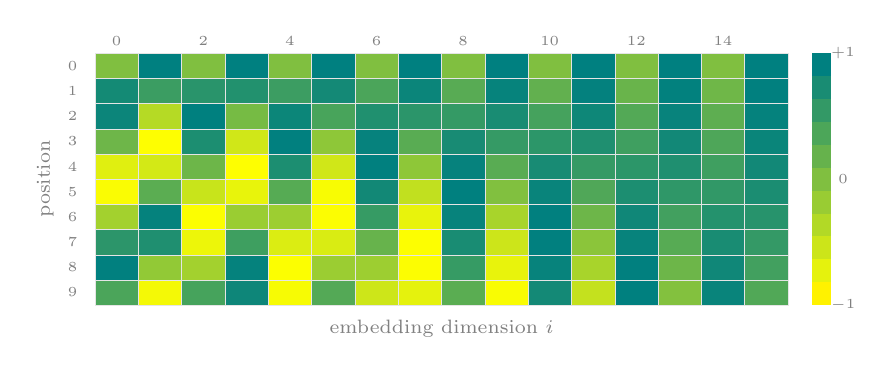
\begin{tikzpicture}[scale=1.0]
    % Heatmap of sinusoidal PE: 10 positions × 16 dimensions
    % Color: sin/cos values mapped to teal (negative) → yellow (positive)
    \def\rows{10}   % positions
    \def\cols{16}   % dimensions shown
    \def\cw{0.55}   % cell width
    \def\ch{0.32}   % cell height

    \foreach \pos in {0,...,9} {
      % row label (position)
      \pgfmathsetmacro{\ry}{(9-\pos)*\ch + \ch/2}
      \node[font=\tiny, gray, anchor=east] at (-0.10, \ry) {\pos};
      \foreach \dimi in {0,...,15} {
        % Compute PE value: even dims → sin, odd dims → cos
        \pgfmathtruncatemacro{\iseven}{mod(\dimi,2) == 0 ? 1 : 0}
        \pgfmathtruncatemacro{\halfdi}{int(\dimi/2)}
        % freq = 10000^(2*halfdi/64) = exp(ln(10000)*2*halfdi/64)
        \pgfmathsetmacro{\freq}{exp(ln(10000)*2*\halfdi/64)}
        \pgfmathsetmacro{\myangle}{\pos / \freq * 180 / 3.14159}
        \pgfmathsetmacro{\peval}{\iseven == 1 ? sin(\myangle) : cos(\myangle)}
        % Map peval from [-1,1] to color percentage
        \pgfmathsetmacro{\colpct}{(\peval + 1) * 50}
        % Precompute rectangle coordinates
        \pgfmathsetmacro{\xa}{\dimi*\cw}
        \pgfmathsetmacro{\ya}{(9-\pos)*\ch}
        \pgfmathsetmacro{\xb}{\dimi*\cw+\cw}
        \pgfmathsetmacro{\yb}{(9-\pos)*\ch+\ch}
        \fill[teal!\colpct!yellow] (\xa, \ya) rectangle (\xb, \yb);
        \draw[gray!20, line width=0.1pt] (\xa, \ya) rectangle (\xb, \yb);
      }
    }

    % Axis labels
    \node[font=\scriptsize, gray, rotate=90, anchor=south] at (-0.40, \rows*\ch/2) {position};
    \node[font=\scriptsize, gray] at (\cols*\cw/2, -0.30) {embedding dimension $i$};

    % Dimension indices at top
    \foreach \dimi in {0,2,...,14} {
      \pgfmathsetmacro{\cx}{\dimi*\cw + \cw/2}
      \node[font=\tiny, gray] at (\cx, \rows*\ch+0.15) {\dimi};
    }

    % Color bar on the right
    \foreach \cb in {0,...,10} {
      \pgfmathsetmacro{\cbval}{\cb * 10}
      \pgfmathsetmacro{\cby}{\cb * \ch * \rows / 11}
      \fill[teal!\cbval!yellow] (\cols*\cw+0.30, \cby) rectangle (\cols*\cw+0.55, \cby + \ch*\rows/11);
    }
    \node[font=\tiny, gray] at (\cols*\cw+0.70, 0) {$-1$};
    \node[font=\tiny, gray] at (\cols*\cw+0.70, \rows*\ch/2) {$0$};
    \node[font=\tiny, gray] at (\cols*\cw+0.70, \rows*\ch) {$+1$};

  \end{tikzpicture}
  \end{center}

  \vspace{-0.3em}
  Modern models use \textbf{learned} positional embeddings or \textbf{RoPE} instead.
\end{frame}

% -----------------------------------------------------------------------
\begin{frame}{Learned Positional Embeddings}

  \textbf{Idea:} Replace the fixed sinusoidal formula with a learnable embedding matrix.

  \vspace{0.5em}
  \begin{itemize}
    \item Embedding table $P \in \R^{L_{\max} \times d}$, initialized randomly
    \item Position $m$ gets embedding $P[m, :]$, added to the token embedding
    \item Trained end-to-end with the rest of the model via backpropagation
  \end{itemize}

  \vspace{0.5em}
  \begin{columns}[T]
    \begin{column}{0.48\textwidth}
      \textbf{Advantages:}
      \begin{itemize}
        \item More expressive: each position has a free embedding
        \item Empirically matches or slightly outperforms sinusoidal PE
        \item Used in GPT-2, BERT, and many early Transformers
      \end{itemize}
    \end{column}
    \begin{column}{0.48\textwidth}
      \textbf{Limitations:}
      \begin{itemize}
        \item Fixed maximum length $L_{\max}$: cannot generalize beyond it
        \item Absolute: attention depends on positions $(m, n)$, not relative distance $m - n$
        \item Adds $L_{\max} \times d$ parameters (modest cost)
      \end{itemize}
    \end{column}
  \end{columns}

\end{frame}

% RoPE and KV-Cache content moved to transformer_advances.tex

